\documentclass[tikz,border=2pt]{standalone}
\renewcommand{\familydefault}{\sfdefault}
\usetikzlibrary{arrows.meta,calc,positioning}
\tikzset{every picture/.style={line width=1pt, >=Stealth},
         hl/.style={fill=black, fill opacity=0.12, text opacity=1}}
\begin{document}
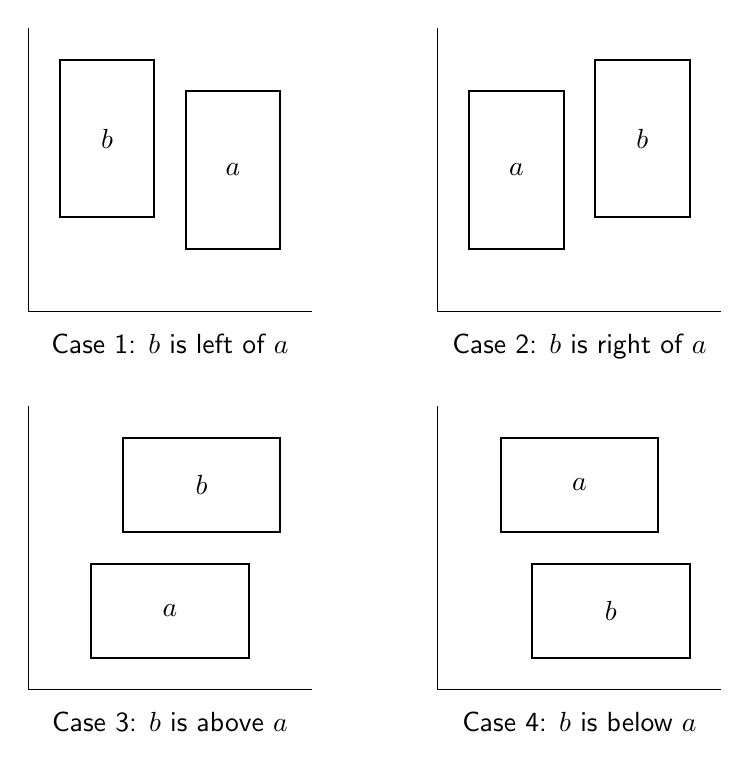
\begin{tikzpicture}[thick, x=0.4cm, y=0.4cm]
  \foreach \dx/\dy/\ax/\aX/\ay/\aY/\bx/\bX/\by/\bY/\txt in {
      0/0/5/8/2/7/1/4/3/8/{Case 1: $b$ is left of $a$},
      13/0/1/4/2/7/5/8/3/8/{Case 2: $b$ is right of $a$},
      0/-12/2/7/1/4/3/8/5/8/{Case 3: $b$ is above $a$},
      13/-12/2/7/5/8/3/8/1/4/{Case 4: $b$ is below $a$}} {
    \begin{scope}[shift={(\dx,\dy)}]
      \draw[thin] (0,9) -- (0,0) -- (9,0);
      \draw (\ax,\ay) rectangle node {$a$} (\aX,\aY);
      \draw (\bx,\by) rectangle node {$b$} (\bX,\bY);
      \node[below] at (4.5,-0.4) {\txt};
    \end{scope}
  }
\end{tikzpicture}
\end{document}
